\documentclass[12pt,a4paper]{book}

\input{../1ere-preambule}

\newcommand{\va}[1]{\lvert \ #1 \ \rvert}
\newcommand{\vaf}[1]{\left\lvert \ #1\  \right\rvert}

\begin{document}
\graphicspath{{images/}}
\setcounter{chapter}{2}
\chapter[Correction des exercices]{Equations et inéquations du second degré \\ correction des exercices}
\thispagestyle{fancy}

\section*{Equation du second degré}

% \subsection*{Ex 18 p 87}

% \begin{enumMet}
%     \item $f(1)=1^2-1+1=1\ne0$. 1 n'est pas une racine.
%     \item $f(-1)=3\times(-1)^2+(-1)-2=0$. $-1$ est 1 racine.
%     \item $f(2)=2\times2^2-3\times2 -2=0$. $2$ est 1 racine.
%     \item $f(3)=-2\times3^2+3+1=-14\ne0$. $3$ n'est pas 1 racine.
% \end{enumMet}

\subsection*{Ex 22 p 87}
\begin{multicols}{2}
\begin{enumMet}
    \item $f(x)=x^2+x-1$\\
    $\Delta=b^2-4ac=1^2-4\times1\times(-1)=5$.\\
    $\Delta>0$ donc 2 racines.
    \item $g(x)=2x^2-x+3$\\
    $\Delta=b^2-4ac=(-1)^2-4\times2\times(3)=-23$.\\
    $\Delta<0$ donc pas de racines.
    \item $h(x)=-5x^2+4x+3$\\
    $\Delta=b^2-4ac=4^2-4\times(-5)\times3=76$.\\
    $\Delta>0$ donc 2 racines.
    \item $j(x)=x^2-\sqrt{2}x+7$\\
    $\Delta=b^2-4ac=\sqrt{2}^2-4\times1\times7=-26$.\\
    $\Delta<0$ donc pas de racines.
\end{enumMet}
\end{multicols}

\subsection*{Ex 23 p 87}
\begin{multicols}{2}
\begin{enumMet}
    \item $x^2+2x-3=0$\\
    $\Delta=b^2-4ac=2^2-4\times1\times(-3)=16$.\\
    $\Delta>0$ donc 2 racines.\\
    $x_1=\dfrac{-b-\sqrt{\Delta}}{2a}=\dfrac{-2-4}{2}=-3$\\
    $x_2=\dfrac{-b+\sqrt{\Delta}}{2a}=\dfrac{-2+4}{2}=1$\\
    $S=\left\{-3;1\right\}$
    \item $x^2-2x-8=0$\\
    $\Delta=b^2-4ac=(-2)^2-4\times1\times(-8)=36$.\\
    $\Delta>0$ donc 2 racines.\\
    $x_1=\dfrac{-b-\sqrt{\Delta}}{2a}=\dfrac{2-6}{2}=-2$\\
    $x_2=\dfrac{-b+\sqrt{\Delta}}{2a}=\dfrac{2+6}{2}=4$\\
    $S=\left\{-2;4\right\}$
    
    \columnbreak
    \item $2x^2+5x-3=0$\\
    $\Delta=b^2-4ac=(5)^2-4\times2\times(-3)=49$.\\
    $\Delta>0$ donc 2 racines.\\
    $x_1=\dfrac{-b-\sqrt{\Delta}}{2a}=\dfrac{-5-7}{4}=-3$\\
    $x_2=\dfrac{-b+\sqrt{\Delta}}{2a}=\dfrac{-5+7}{4}=\dfrac{1}{2}$\\
    $S=\left\{-3;\dfrac{1}{2}\right\}$
    \item $x^2-2x+1=0$\\
    $\Delta=b^2-4ac=(-2)^2-4\times1\times1=0$.\\
    $\Delta=0$ donc 1 racine double.\\
    $x_0=\dfrac{-b}{2a}=\dfrac{2}{2}=1$\\
    $S=\left\{1\right\}$
\end{enumMet}
\end{multicols}

\newpage

\subsection*{Ex 25 p 87}
\begin{multicols}{2}
\begin{enumMet}
    \item $3x^2+4x+5=0$\\
    $\Delta=b^2-4ac=4^2-4\times3\times(5)=-44$.\\
    $\Delta<0$ donc aucune solution réelle.\\
    $S=\varnothing$
    \item $-3x^2+11x+4=0$\\
    $\Delta=b^2-4ac=11^2-4\times(-3)\times4=169$.\\
    $\Delta>0$ donc 2 racines.\\
    $x_1=\dfrac{-b-\sqrt{\Delta}}{2a}=\dfrac{-11-13}{-6}=4$\\
    $x_2=\dfrac{-b+\sqrt{\Delta}}{2a}=\dfrac{-11+13}{-6}=-\dfrac{1}{3}$\\
    $S=\left\{-\dfrac{1}{3};4\right\}$
    
    \columnbreak
    \item $2x^2-2x-3=0$\\
    $\Delta=b^2-4ac=(-2)^2-4\times2\times(-3)=28$.\\
    $\Delta>0$ donc 2 racines.\\
    $x_1=\dfrac{-b-\sqrt{\Delta}}{2a}=\dfrac{2-\sqrt{28}}{4}=\dfrac{1-\sqrt{7}}{2}$\\
    $x_2=\dfrac{-b+\sqrt{\Delta}}{2a}=\dfrac{2+\sqrt{28}}{4}=\dfrac{1+\sqrt{7}}{2}$\\
    $S=\left\{\dfrac{1-\sqrt{7}}{2};\dfrac{1+\sqrt{7}}{2}\right\}$
    \item $x^2-2x-2=0$\\
    $\Delta=b^2-4ac=(-2)^2-4\times1\times(-2)=12$.\\
    $\Delta>0$ donc 2 racines.\\
    $x_1=\dfrac{-b-\sqrt{\Delta}}{2a}=\dfrac{2-\sqrt{12}}{2}=1-\sqrt{3}$\\
    $x_2=\dfrac{-b+\sqrt{\Delta}}{2a}=\dfrac{2+\sqrt{12}}{2}=1+\sqrt{3}$\\
    $S=\left\{1-\sqrt{3};1+\sqrt{3}\right\}$
\end{enumMet}
\end{multicols}

\subsection*{Ex 26 p 87}
\begin{multicols}{2}
\begin{enumMet}
    \item $2x^2+4x+2=0$\\
    $\Delta=4^2-4\times2\times2=0$.\\
    $\Delta=0$ donc 1 solution réelle.\\
    $x_0=-\dfrac{b}{2a}=-\dfrac{4}{4}=-1$\\
    $S=\left\{-1\right\}$\\
    On pouvait aussi passer par l'I.R:\\
    $2x^2+4x+2=0\iff 2(x+1)^2=0\iff ...$
    \item $-3x^2+4x+2=0$\\
    $\Delta=4^2-4\times(-3)\times2=40$.\\
    $\Delta>0$ donc 2 racines.\\
    $x_1=\dfrac{-b-\sqrt{\Delta}}{2a}=\dfrac{-4-\sqrt{40}}{-6}=\dfrac{2+\sqrt{10}}{3}$\\
    $x_2=\dfrac{-b+\sqrt{\Delta}}{2a}=\dfrac{-4+\sqrt{40}}{-6}=\dfrac{2-\sqrt{10}}{3}$\\
    $S=\left\{\dfrac{2-\sqrt{10}}{3};\dfrac{2+\sqrt{10}}{3}\right\}$
    
    \columnbreak
    \item $3x^2+12x-15=0$\\
    $\Delta=12^2-4\times3\times(-15)=324$.\\
    $\Delta>0$ donc 2 racines.\\
    $x_1=\dfrac{-b-\sqrt{\Delta}}{2a}=\dfrac{-12-\sqrt{324}}{6}=-5$\\
    $x_2=\dfrac{-b+\sqrt{\Delta}}{2a}=\dfrac{-12+\sqrt{324}}{6}=1$\\
    $S=\left\{-5;1\right\}$
    \item $7x^2-x-2=0$\\
    $\Delta=b^2-4ac=(-1)^2-4\times7\times(-2)=57$.\\
    $\Delta>0$ donc 2 racines.\\
    $x_1=\dfrac{-b-\sqrt{\Delta}}{2a}=\dfrac{1-\sqrt{57}}{14}$\\
    $x_2=\dfrac{-b+\sqrt{\Delta}}{2a}=\dfrac{1+\sqrt{57}}{14}$\\
    $S=\left\{\dfrac{1-\sqrt{57}}{14};\dfrac{1+\sqrt{57}}{14}\right\}$
\end{enumMet}
\end{multicols}

\newpage

\subsection*{Ex 31 p 87}
\begin{enumMet}
    \item $f(x)=x^{2}-4 x+1$\\
    On a $\Delta=(-4)^{2}-4 \times 1 \times 1=12$.\\
    On calcule ensuite les coordonnées du sommet de la parabole grâce aux formules suivantes :\\
    $\alpha=-\dfrac{b}{2 a}=-\dfrac{-4}{2 \times 1}=2$ et $\beta=-\dfrac{\Delta}{4 a}=-\dfrac{12}{4 \times 1}=-3$.\\
    Donc le sommet de la parabole représentant le trinôme a pour coordonnées $(2 ;-3)$.\\
    On peut aussi utiliser $\alpha=\dfrac{x_1+x_2}{2}$ et $\beta=f(\alpha)=2^2-4\times2+1$
    \item $f(x)=-x^{2}+x-1$\\
    De même on obtient que $\Delta=-3$ et que le sommet a pour coordonnées $\left(\dfrac{1}{2} ;-\dfrac{3}{4}\right)$.
    \item $f(x)=2 x^{2}-4 x+5$\\
    De même on obtient que $\Delta=-24$ et que le sommet a pour coordonnées $(1 ; 3)$.
    \item  $f(x)=-3 x^{2}+7 x+2$\\
    De même on obtient que $\Delta=73$ et que le sommet a pour coordonnées $\left(\dfrac{7}{6} ; \dfrac{73}{12}\right)$.
    \item $f(x)=5 x^{2}+x-3$\\
    De même on obtient que $\Delta=61$ et que le sommet a pour coordonnées $\left(-\dfrac{1}{10} ;-\dfrac{61}{20}\right)$.
\end{enumMet}

\subsection*{Ex 40 p 88}
\begin{multicols}{2}
\begin{enumMet}
    \item $\dfrac{1}{3} x^{2}-x-1=0$\\
    $\Delta=(-1)^{2}-4 \times \dfrac{1}{3} \times(-1)=\dfrac{7}{3}$.\\
    $\Delta>0$ donc 2 racines.\\
    $x_{1}=\dfrac{1-\sqrt{\dfrac{7}{3}}}{\dfrac{2}{3}}=\dfrac{3}{2} \times\left(1-\sqrt{\dfrac{7}{3}}\right)=\dfrac{\sqrt{3}}{2}(\sqrt{3}-\sqrt{7})$\\
    $x_{2}=\dfrac{1+\sqrt{\dfrac{7}{3}}}{2 \times \dfrac{1}{3}}=\dfrac{3}{2} \times\left(1+\sqrt{\dfrac{7}{3}}\right)=\dfrac{\sqrt{3}}{2}(\sqrt{3}+\sqrt{7})$\\
    $S=\left\{\dfrac{\sqrt{3}}{2}(\sqrt{3}-\sqrt{7});\dfrac{\sqrt{3}}{2}(\sqrt{3}+\sqrt{7})\right\}$\\
    \item $-x^{2}+\sqrt{3} x+3=0$\\
    $\Delta=(\sqrt{3})^{2}-4 \times(-1) \times 3=15$.\\
    $\Delta>0$ donc 2 racines.\\
    $x_{1}=\dfrac{-\sqrt{3}-\sqrt{15}}{-2}=\dfrac{\sqrt{3}+\sqrt{15}}{2}$\\
    $x_{2}=\dfrac{\sqrt{3}-\sqrt{15}}{2}$\\
    $S=\left\{\dfrac{\sqrt{3}-\sqrt{15}}{2};\dfrac{\sqrt{3}+\sqrt{15}}{2}\right\}$
    
    \columnbreak
    \item $\dfrac{(2 x-1)^{2}}{2}=3$\\
    On commence par réécrire l'équation pour la mettre sous la forme d'un trinôme égal à 0 : \\
    $\dfrac{(2 x-1)^{2}}{2}=3 \Leftrightarrow \dfrac{4 x^{2}-4 x+1}{2}=3 \Leftrightarrow 4 x^{2}-4 x+1=6 \Leftrightarrow 4 x^{2}-4 x-5=0$
    $\Delta=(-4)^{2}-4 \times 4 \times(-5)=96$\\
    $\Delta>0$ donc 2 racines.\\
    $x_{1}=\dfrac{4-\sqrt{96}}{2 \times 4}=\dfrac{1-\sqrt{6}}{2}$\\
    $x_{2}=\dfrac{1+\sqrt{6}}{2}$\\
    $S=\left\{\dfrac{1-\sqrt{6}}{2};\dfrac{1+\sqrt{6}}{2}\right\}$
    \item $-2 x^{2}+\dfrac{x}{4}=1$\\
    On commence par réécrire l'équation pour la mettre sous la forme d'un trinôme égal à 0 : \\
    $-2 x^{2}+\dfrac{x}{4}=1 \Leftrightarrow-8 x^{2}+x-4=0$\\
    $\Delta=1^{2}-4 \times(-8) \times(-4)=-127$\\
    $\Delta<0$ donc aucune solution réelle.\\
    $S=\varnothing$
\end{enumMet}
\end{multicols}


\subsection*{Ex 42 p 88}
\begin{enumMet}
    \item $x^{2}-3=0$\\
    $x^{2}=3$\\
    $x=\sqrt{3}$ ou $x=-\sqrt{3}$
    $S=\left\{-\sqrt{3};+\sqrt{3}\right\}$\\
    \item $2 x^{2}+5=0$\\
    $x^{2}=-\dfrac{5}{2}$\\
    un carré est toujours $>0$.\\
    $S=\varnothing$
    \item $x^{2}=3 x+1$\\
    On commence par réécrire l'équation pour la mettre sous la forme d'un trinôme égal à 0 : \\
    $x^{2}=3 x+1 \Leftrightarrow x^{2}-3 x-1=0$\\
    $\Delta=(-3)^{2}-4 \times 1 \times(-1)=13$\\
    $\Delta>0$ donc 2 racines.\\
    $x_{1}=\dfrac{3-\sqrt{13}}{2}$\\
    $x_{2}=\dfrac{3+\sqrt{13}}{2}$\\
    $S=\left\{\dfrac{3-\sqrt{13}}{2};\dfrac{3+\sqrt{13}}{2}\right\}$
    \item $x-3 x^{2}=0$\\
    $x-3 x^{2}=0 \Leftrightarrow x(1-3 x)=0 \Leftrightarrow x=0$ ou $1-3 x=0$ d'après la règle du produit nul.\\
    Donc l'équation admet deux solutions $x_{1}=0$ et $x_{2}=\dfrac{1}{3}$\\
    $S=\left\{0;\dfrac{1}{3}\right\}$
    \item $4 x^{2}+8 x-12=0$\\
    On peut tout d'abord simplifier l'équation :\\
    $4 x^{2}+8 x-12=0 \Leftrightarrow 4\left(x^{2}+2 x-3\right)=00 \Leftrightarrow x^{2}+2 x-3=0$\\
    $\Delta=2^{2}-4 \times 1 \times(-3)=16$.\\
    $\Delta>0$ donc 2 racines.\\
    $x_{1}=\dfrac{-2-\sqrt{16}}{2}=-3$\\
    $x_{2}=\dfrac{-2+\sqrt{16}}{2}=1$\\
    $S=\left\{-3;1\right\}$
    \item $9(x+1)^{2}-(2 x+3)^{2}=0$\\
    On commence par écrire cette équation sous la forme d'un trinôme égal à 0 :\\
    $$
    \begin{aligned}
    9(x+1)^{2}-(2 x+3)^{2}=0 & \Leftrightarrow 9\left(x^{2}+2 x+1\right)-\left(4 x^{2}+12 x+9\right)=0 \\
    & \Leftrightarrow 5 x^{2}+6 x=0 \\
    & \Leftrightarrow x(5 x+6)=0
    \end{aligned}
    $$
    Donc, d'après la règle du produit nul, soit $x=0$ soit $5 x+6=0$ donc l'équation admet deux solutions $x_{1}=0$ et $x_{2}=-\dfrac{6}{5}$\\
\end{enumMet}

% \subsection*{Ex 45 p 89}

% \begin{enumMet}
%     \item $x-\dfrac{1}{x}=3$\\
%     On résout l'équation dans $\mathbb{R}^{*}$ car le dénominateur de $\dfrac{1}{x}$ ne doit pas s'annuler. On commence par écrire différemment l'équation, de manière à faire apparaitre un trinôme du second degré :\\
%     $x-\dfrac{1}{x}=3 \Leftrightarrow x-\dfrac{1}{x}-3=0 \Leftrightarrow \dfrac{x^{2}-3 x-1}{x}=0$.\\ 
%     Résoudre cette équation revient donc à résoudre l'équation $x^{2}-3 x-1=0 .$\\ 
%     On calcule le discriminant:\\
%     $\Delta=(-3)^{2}-4 \times 1 \times(-1)=13>0$\\ 
%     L'équation $x^{2}-3 x-1=0$ admet donc deux solutions réelles distinctes:\\
%     $x_{1}=\dfrac{3-\sqrt{13}}{2}$ et $x_{2}=\dfrac{3+\sqrt{13}}{2}$.\\ 
%     Aucune n'est nulle donc l'équation $x-\dfrac{1}{x}=3$ admet elle aussi deux solutions réelles distinctes:\\ $x_{1}=\dfrac{3-\sqrt{13}}{2}$ et $x_{2}=\dfrac{3+\sqrt{13}}{2}$
%     \item $\dfrac{x+1}{2}+\dfrac{1}{x-4}=1$\\
%     On résout l'équation dans $\mathbb{R} \backslash\{4\}$ car le dénominateur de $\dfrac{1}{x-4}$ ne doit pas s'annuler.\\ 
%     On commence par écrire différemment l'équation, de manière à faire apparaitre un trinôme du second degré :\\
%     $$
%     \dfrac{x+1}{2}+\dfrac{1}{x-4}=1 \Leftrightarrow \dfrac{(x+1)(x-4)+2}{2(x-4)}=1 \Leftrightarrow \dfrac{x^{2}-5 x+6}{2(x-4)}=0
%     $$
%     Résoudre cette équation revient donc à résoudre l'équation $x^{2}-5 x+6=0 .$\\ 
%     On calcule le discriminant :\\ 
%     $\Delta=(-5)^{2}-4 \times 1 \times 6=1>0$\\ 
%     L'équation admet donc deux solutions: \\
%     $x_{1}=\dfrac{5-\sqrt{1}}{2}=2$  et ${x_{2}}=\dfrac{5+\sqrt{1}}{2}=3$\\
%     Aucune n'est égale à 4 donc l'équation $\dfrac{x+1}{2}+\dfrac{1}{x-4}=1$ admet elle aussi deux solutions réelles distinctes : $2$ et $3$.
%     \item $\dfrac{1}{x}+\dfrac{1}{x+2}=4$\\
%     On résout l'équation dans $\mathbb{R} \backslash\{-2 ; 0\}$. On doit exclure -2 pour que le dénominateur de
%     $\dfrac{1}{x+2}$ ne risque pas s'annuler et on doit exclure 0 afin que le dénominateur de $\dfrac{1}{x}$ ne risque pas de s'annuler non plus.\\
%     On commence par écrire différemment l'équation, de manière à faire apparaître un trinôme du second degré:\\
%     $\dfrac{1}{x}+\dfrac{1}{x+2}=4 \Leftrightarrow \dfrac{x+2+x}{x(x+2)}=4 \Leftrightarrow \dfrac{-4 x^{2}-6 x+2}{x(x+2)}=0$\\
%     Résoudre l'équation revient donc à résoudre l'équation $-4 x^{2}-6 x+2=0 .$\\
%     On calcule le discriminant:\\
%     $\Delta=(-6)^{2}-4 \times(-4) \times 2=68>0$\\
%     L'équation admet donc deux solutions réelles distinctes:\\
%     $x_{1}=\dfrac{6-\sqrt{68}}{-8}=\dfrac{\sqrt{17}-3}{4}$ et $x_{2}=\dfrac{-3-\sqrt{17}}{4}$.\\
%     Aucune de ces solutions n'est égale à $0$ ou à $-2$ donc l'équation $\dfrac{1}{x}+\dfrac{1}{x+2}=4$ admet elle aussi deux solutions réelles distinctes: $\dfrac{\sqrt{17}-3}{4}$ et $\dfrac{-3-\sqrt{17}}{4}$.
% \end{enumMet}


% \subsection*{Ex 43 p 88}
% \begin{enumMet}
%     \item $5 x(2-3 x)=4-9 x^{2}$\\
%     En utilisant une identité remarquable, on peut réécrire l'équation ainsi :\\
%     $$
%     \begin{aligned}
%     5 x(2-3 x)=4-9 x^{2} & \Leftrightarrow 5 x(2-3 x)=(2-3 x)(2+3 x) \text { ), Et donc, } \\
%     5 x(2-3 x)=4-9 x^{2} & \Leftrightarrow 5 x(2-3 x)-(2-3 x)(2+3 x)=0 \\
%     & \Leftrightarrow(2-3 x)(5 x-(2+3 x))=0 \\
%     & \Leftrightarrow(2-3 x)(2 x-2)=0
%     \end{aligned}
%     $$
%     Donc, d'après la règle du produit nul, soit $2-3 x=0,$ soit $2 x-2=0$ L'équation admet donc deux solutions réelles:\\
%     $x_{1}=\dfrac{2}{3}$ et $x_{2}=1$.
    
%     \item $12 x^{2}+12 x+3=0$\\
%     On peut tout d'abord simplifier l'équation en divisant par 3:\\
%     $12 x^{2}+12 x+3=0 \Leftrightarrow 4 x^{2}+4 x+1=0$\\
%     On peut ensuite reconnaître une identité remarquable pour réécrire encore plus l'équation :\\
%     $(2 x+1)^{2}=0 $\\
%     Enfin, de part la règle du produit nul, on a que $2 x+1=0$ et donc que l'équation admet une seule solution réelle:\\
%     $x_{0}=-\dfrac{1}{2}$
%     \item $3(x+5)^{2}=48$\\
%     On peut tout d'abord simplifier cette équation en divisant à gauche et à droite par 3 :\\
%     $3(x+5)^{2}=48 \Leftrightarrow(x+5)^{2}=16$\\
%     En écrivant maintenant l'équation ainsi : $(x+5)^{2}-16=0$, on peut reconnaître une identité remarquable qui nous permet d'écrire l'équation sous la forme suivante :\\
%     $(x+5-4)(x+5+4)=0$ c'est à dire $(x+1)(x+9)=0$.\\
%     Donc, d'après la règle du produit nul, $x+1=0$ ou $x+9=0 .$ L'équation admet donc deux solutions réelles:\\
%     $x_{1}=-1$ et $x_{2}=-9$
%     \item $2(x-3)^{2}+(2 x-7)^{2}=0$\\
%     Pour tout $x \in \R$, $2(x-3)^2 \geq 0$ et $(2 x-7)^2 \geq 0$.\\
%     Or, la somme de deux nombres positifs ou nuls est égale à zéro si, et seulement si, les deux nombres sont égaux à zéro.\\
%     Donc on doit avoir $2(x-3)^{2}=0$ et $(2 x-7)^{2}=0$, c'est à dire qu'on doit avoir $x=3$ et $x=\dfrac{7}{2}$.\\
%     Or $x$ ne peut pas être égal en même temps à 3 et à $x=\dfrac{7}{2}$. Donc l'équation n'admet pas de solution dans $\mathbb{R}$.\\
%     $S=\varnothing$
%     \item $8 x^{3}+5=(2 x-3)^{3}-(x+1)^{2}$\\
%     On commence par écrire cette équation sous la forme d'un trinôme égal à 0 :
%     $$
%     \begin{aligned}
%     8 x^{3}+5=(2 x-3)^{3}-(x+1)^{2} & \Leftrightarrow 8 x^{3}+5=8 x^{3}-36 x^{2}+54 x-27-\left(x^{2}+2 x+1\right) \\
%     & \Leftrightarrow 8 x^{3}+5=8 x^{3}-37 x^{2}+52 x-28 \\
%     & \Leftrightarrow 37 x^{2}-52 x+33=0
%     \end{aligned}
%     $$
%     Puis on calcule son discriminant : $\Delta=(-52)^{2}-4 \times 37 \times 33=-2180$, On a $\Delta<0$ donc l'équation n'admet pas de solution dans $\mathbb{R}$
%     \item $(x-1)\left(x^{2}+2\right)-(2 x-2)\left(-x^{2}+5 x-1\right)=0$\\
%     On peut commencer par simplifier l'écriture de cette équation:\\
%     $(x-1)\left(x^{2}+2\right)-(2 x-2)\left(-x^{2}+5 x-1\right)=0$
%     $\Leftrightarrow(x-1)\left(x^{2}+2\right)-2(x-1)\left(-x^{2}+5 x-1\right)=0$
%     $\Leftrightarrow(x-1)\left(3 x^{2}-10 x+4\right)=0$\\
%     Donc, d'après la règle du produit nul, soit $x-1=0,$ soit $3 x^{2}-10 x+4=0$.\\
%     Donc on sait déjà que $x=1$ est une solution de cette équation. Pour trouver les potentielles autres solutions de cette équation on doit résoudre l'équation $3 x^{2}-10 x+4=0$.\\
%     Calculons le discriminant pour cette deuxième équation : \\
%     $\Delta=(-10)^{2}-4 \times 3 \times 4=52$.\\
%     On a $\Delta \geq 0$ donc l'équation admet deux solutions réelles distinctes:\\ $x_{1}=\dfrac{10-\sqrt{52}}{6}=\dfrac{5-\sqrt{13}}{3}$ et \\
%     $x_{2}=\dfrac{5+\sqrt{13}}{3}$.\\
%     En conclusion l'équation admet trois solutions: 1; $\dfrac{5-\sqrt{13}}{3}$ et $\dfrac{5+\sqrt{13}}{3}$
% \end{enumMet}

% \subsection*{Ex 47 p 89}

% \begin{enumMet}
%     \item $f: x \mapsto \dfrac{1}{2 x^{2}+3 x-5}$\\
%     Chercher le domaine de définition de $f$ revient à résoudre $2 x^{2}+3 x-5=0$. On calcule le discriminant : $\Delta=3^{2}-4 \times 2 \times(-5)=49>0$ donc l'équation admet deux solutions réelles distinctes :\\
%     $x_{1}=\dfrac{-3-\sqrt{49}}{4}=-\dfrac{5}{2}$ et $x_{2}=\dfrac{-3+\sqrt{49}}{4}=1$.\\
%     Donc $f$ est définie partout sauf là où son dénominateur s'annule, c'est à dire sur $\R\backslash\left\{\dfrac{-5}{2} ; 1\right\}$
%     \item $g: x \rightarrow \dfrac{7-x}{-x^{2}+x-3}$\\
%     Chercher le domaine de définition de $g$ revient à résoudre $-x^{2}+x-3=0$.\\
%     On calcule le discriminant $: \Delta=1^{2}-4 \times(-1) \times(-3)=-11<0$ donc l'équation n'admet pas de solution réelle. Donc $g$ est définie sur $\mathbb{R}$.
%     \item $h: x \mapsto \dfrac{3}{4 x^{3}-x^{2}-3 x}$\\
%     Chercher le domaine de définition de $h$ revient à résoudre $4 x^{3}-x^{2}-3 x=0 .$\\
%     On a $4 x^{3}-x^{2}-3 x=0 \Leftrightarrow x\left(4 x^{2}-x-3\right)=0$ donc, d'après la règle du produit nul, pour que ce produit s'annule on doit soit avoir $x=0,$ soit avoir $4 x^{2}-x-3=0$.\\
%     On calcule le discriminant $\Delta$ de la deuxième équation:\\
%     $\Delta=(-1)^{2}-4 \times 4 \times(-3)=49>0$ donc l'équation admet deux solutions réelles distinctes:\\
%     $x_{1}=\dfrac{1-\sqrt{49}}{8}=-\dfrac{3}{4}$ et $x_{2}=\dfrac{1+\sqrt{49}}{8}=1$. Donc l'équation $4 x^{3}-x^{2}-3 x=0$ admet 3 solutions réelles $: 0,-\dfrac{3}{4}$ et $1$ . Donc $h$ est définie sur $\mathbb{R} \backslash\left\{-\dfrac{3}{4} ; 0 ; 1\right\}$
%     \item $\ell: x \mapsto \dfrac{\sqrt{x}}{x^{2}+x-5}$\\
%     Pour trouver le domaine de définition de la fonction $\ell$ on commence par résoudre l'équation $x^{2}+x-5=0$.\\
%     En calculant le discriminant on obtient $\Delta=1^{2}-4 \times 1 \times(-5)=21$ 
%     Donc $\Delta>0$ donc l'équation admet deux solutions réelles distinctes:\\
%     $x_{1}=\dfrac{-1-\sqrt{21}}{2}$ et $x_{2}=\dfrac{-1+\sqrt{21}}{2}$. \\
%     De plus, la fonction racine carrée existe si, et seulement si, $x \geq 0$. Donc $\ell$ est définie sur l'ensemble : $\left[0 ; \dfrac{-1+\sqrt{21}}{2}\right[\cup\left] \dfrac{-1+\sqrt{21}}{2} ;+\infty\right[.$
% \end{enumMet}

% \section*{Somme et produit de racines}





 \subsection*{Ex 80 p 93}

 \begin{enumMet}
     \item 1 est une solution évidente de $2 x^{2}+x-3=0 .$ On appelle $x_{2}$ l'autre solution.\\
    
     On sait que lorsqu' un trinôme $a x^{2}+b x+c$ admet deux racines distinctes ou confondues leur somme $S$ et leur produit $P$ vérifient $: S=-\dfrac{b}{a}$ et $P=\dfrac{c}{a}$.\\
    
     On a donc ici $1 \times x_{2}=\dfrac{-3}{2}$. Donc $x_{2}=\dfrac{-3}{2}$.
     \item -1 est une solution évidente de $3 x^{2}+10 x+7=0 .$ On appelle $x_{2}$ l'autre solution. \\
    
     Pour les mêmes raisons on a $-1 \times x_{2}=\dfrac{7}{3}$. Donc $x_{2}=-\dfrac{7}{3}$
     \item 1 est une solution évidente de $x^{2}+(\sqrt{3}-1) x-\sqrt{3}=0 .$ On appelle $x_{2}$ l'autre solution.\\
    
     Pour les mêmes raisons on a $1 \times x_{2}=-\sqrt{3}$. Donc $x_{2}=-\sqrt{3}$.
     \item $\sqrt{5}$ est une solution évidente de $x^{2}+4 \sqrt{5} x-25=0 .$ On appelle $x_{2}$ l'autre solution.\\
    
     Pour les mêmes raisons on a $\sqrt{5} \times x_{2}=\dfrac{-25}{1}$. Donc $x_{2}=-\dfrac{25}{\sqrt{5}}=-5 \sqrt{5}$
 \end{enumMet}

% \subsection*{Ex 81 p 93}

% Deux réels ont pour somme 10 et pour produit $13$ si, et seulement si, ils sont solutions de l'équation $x^{2}-10 x+13=0 .$ \\
% $ax^2+bx+c = 0 \iff x^2+\dfrac{b}{a}x+\dfrac{c}{a}=0 \iff x^2-Sx+P=0$
% Le discriminant de ce trinôme vaut $\Delta=48>0,$ l'équation admet donc deux solutions réelles distinctes:\\

% $x_{1}=\dfrac{10-\sqrt{48}}{2}=5-2 \sqrt{3}$ et $x_{2}=\dfrac{10+\sqrt{48}}{2}=5+2 \sqrt{3}$\\

% On peut vérifier qu'on a bien $x_{1}+x_{2}=10$ et $x_{1} x_{2}=5^{2}-(2 \sqrt{3})^{2}=25-12=13$

\section*{Équation du second degré}

% \subsection*{Ex 36 p 88}

% \begin{enumMet}
%     \item On peut réécrire $x^{2}-16=0$ en $x^{2}=16$. L'équation a donc deux solutions : $4$ et $-4$ .
%     \item On peut réécrire $x^{2}+1=0$ en $x^{2}=-\dfrac{1}{2}$. Or un carré ne peut pas être négatif, cette équation n'a donc aucune solution.
%     \item On peut réécrire $2 x^{2}=18$ en $x^{2}=9$. L'équation a donc deux solutions : $3$ et $-3$ .
%     \item On peut réécrire $4 x^{2}=12$ en $x^{2}=3$. L'équation a donc deux solutions $: \sqrt{3}$ et $-\sqrt{3}$.
%     \item On peut réécrire $x^{2}-x=0$ en $x(x-1)=0$. L'équation a donc deux solutions : 0 et 1.
%     \item On peut réécrire $4 x^{2}-1=0$ en $x^{2}=\dfrac{1}{4}$. L'équation a donc deux solutions: $\dfrac{1}{2}$ et $-\dfrac{1}{2}$.
% \end{enumMet}


\subsection*{Ex 27 p 87}

\begin{enumMet}
    \item $f(x)=x^{2}-6 x-7$\\
    $\Delta=(-6)^{2}-4 \times 1 \times(-7)=64$\\
    $\Delta>0$ donc l'équation admet deux solutions réelles.\\ $x_{1}=\dfrac{6-\sqrt{64}}{2}=-1$ et $x_{2}=\dfrac{6+\sqrt{64}}{2}=7$.\\ 
    Donc $f(x)=a(x-x_1)(x-x_2)=(x+1)(x-7)$
    \item $f(x)=-x^{2}+2 x+8$\\
    $\Delta=2^{2}-4 \times(-1) \times 8=36$ \\
    $\Delta>0$ donc l'équation admet deux solutions réelles.\\
    $x_{1}=\dfrac{-2-\sqrt{36}}{-2}=4$ et $x_{2}=\dfrac{-2+\sqrt{36}}{-2}=-2$. \\
    Donc $f(x)=-(x+2)(x-4)$ pour tout $x \in \mathbb{R}$
    \item $f(x)=-3 x^{2}+5 x+2$\\
    $\Delta=5^{2}-4 \times(-3) \times 2=49$ \\
    $\Delta>0$ donc l'équation admet deux solutions réelles.\\
    $x_{1}=\dfrac{-5-\sqrt{49}}{-6}=2 $ et $x_{2}=\dfrac{-5+\sqrt{49}}{-6}=-\dfrac{1}{3}$.\\
    Donc $f(x)=-3(x-2)\left(x+\dfrac{1}{3}\right)=(x-2)(-3 x-1)$ 
    \item $f(x)=3 x^{2}+x+4$\\
    $\Delta=1^{2}-4 \times 3 \times 4=-47$\\
    $\Delta<0$ donc $f$ n'admet aucune racine réelle.\\
    Donc $f$ n'est pas factorisable dans $\mathbb{R}$.
    \item $f(x)=-4 x^{2}+28 x-49$\\
    On a, pour tout $x \in \mathbb{R}$: \\
    $f(x)=-4 x^{2}+28 x-49=-\left(4 x^{2}-28 x+49\right)=-(2 x-7)^{2}$\\
    Donc $f(x)=-(2 x-7)^{2}$ pour tout $x \in \mathbb{R}$
    \item $f(x)=x^{2}-x-1$\\
    On a $\Delta=(-1)^{2}-4 \times 1 \times(-1)=5$\\
    $\Delta>0$ donc l'équation admet deux solutions réelles.\\
    $x_{1}=\dfrac{1-\sqrt{5}}{2}$ et $x_{2}=\dfrac{1+\sqrt{5}}{2}$\\
    Donc $f(x)=\left(x-\dfrac{1-\sqrt{5}}{2}\right)\left(x-\dfrac{1+\sqrt{5}}{2}\right)$
\end{enumMet}

\subsection*{Ex 29 p 87}

\begin{enumMet}
    \item $f(x)=x^{2}-x-2$\\
    $S=-\dfrac{b}{a}=\dfrac{1}{1}=1$ et $P=\dfrac{c}{a}=\dfrac{-2}{1}=-2$
    \item $f(x)=x^{2}+3 x+1$\\
    $S=-\dfrac{b}{a}=\dfrac{-3}{1}=-3$ et $P=\dfrac{c}{a}=\dfrac{1}{1}=1$
    \item $f(x)=-x^{2}+5 x+2$\\
    $S=-\dfrac{b}{a}=\dfrac{-5}{-1}=5$ et $P=\dfrac{c}{a}=\dfrac{2}{-1}=-2$
    \item $f(x)=2 x^{2}+7 x-1$\\
    $S=-\dfrac{b}{a}=\dfrac{-7}{2}=-\dfrac{7}{2}$ et $P=\dfrac{c}{a}=\dfrac{-1}{2}=-\dfrac{1}{2}$
    \item $f(x)=-3 x^{2}+11 x+7$
    $S=-\dfrac{b}{a}=-\dfrac{11}{-3}=\dfrac{11}{3}$ et $P=\dfrac{c}{a}=\dfrac{7}{-3}=-\dfrac{7}{3}$
\end{enumMet}

\subsection*{Ex 30 p 87}

\begin{enumMet}
    \item $f(x)=9x^{2}+x-1$\\
    $S=-\dfrac{b}{a}=-\dfrac{1}{9}$ et $P=\dfrac{c}{a}=-\dfrac{1}{9}$
    \item $f(x)=-x^{2}-\sqrt{2} x+3$\\
    $S=-\dfrac{b}{a}=-\dfrac{-\sqrt{2}}{-1}=-\sqrt{2}$ et $P=\dfrac{c}{a}=\dfrac{3}{-1}=-3$
    \item $f(x)=\sqrt{3}x^{2}+2 x-1$\\
    $S=-\dfrac{b}{a}=\dfrac{-2}{\sqrt{3}}=-\dfrac{2\sqrt{3}}{3}$ et $P=\dfrac{c}{a}=\dfrac{-1}{\sqrt{3}}=-\dfrac{\sqrt{3}}{3}$
    \item $f(x)=-\sqrt{3}x^{2}-3\sqrt{5}x+1$\\
    $S=-\dfrac{b}{a}=-\dfrac{-3\sqrt{5}}{-\sqrt{3}}=-\sqrt{15}$ et $P=\dfrac{c}{a}=\dfrac{1}{-\sqrt{3}}=-\dfrac{\sqrt{3}}{3}$
    \item $f(x)=5x^{2}+\pi x-3$\\
    $S=-\dfrac{b}{a}=-\dfrac{\pi}{5}$ et $P=\dfrac{c}{a}=\dfrac{-3}{5}=-\dfrac{3}{5}$
\end{enumMet}

\subsection*{Ex 61 p 91}
\grasInMet{On pose $\mathrm{A}(x)=\frac{x+1}{x^2-3 x-4}$}
\begin{enumMet}
    \item \grasInMet{Déterminer les racines de $x^2-3 x-4$.}\\
    On commence par calculer le discriminant : $\Delta=(-3)^{2}-4 \times 1 \times(-4)=25$.\\
    Comme $\Delta>0$, cette équation admet deux racines réelles : $x_{1}=\dfrac{3-\sqrt{25}}{2}=-1$ et $x_{2}=\dfrac{3+\sqrt{25}}{2}=4$
    \item \grasInMet{Factoriser $x^2-3 x-4$.}\\ 
    Grâce à la question précédente on sait que $-1$ et 4 sont racines de $x^{2}-3 x-4 .$ Ce polynôme peut donc être mis sous la forme factorisée suivante : $(x+1)(x-4)$.
    \item \grasInMet{Après avoir précisé l'ensemble des réels $x$ pour lesquels $\mathrm{A}(x)$ existe, simplifier l'écriture de $\mathrm{A}(x)$.}\\ 
    $A$ est définie sur $\mathbb{R} \backslash\{-1 ; 4\}$ car si $x=1$ ou $x=4$, le dénominateur de cette fonction s'annule, on doit donc exclure ces deux valeurs.\\
    Et, au final, pour tout $x \in \mathbb{R} \backslash\{-1 ; 4\}$ on a :\\
    $A(x)=\dfrac{x+1}{(x+1)(x-4)}=\dfrac{1}{x-4}$
\end{enumMet}


\subsection*{Ex 63 p 91}
\grasInMet{Reprendre l'exercice précédent avec les fractions rationnelles suivantes.}
\begin{enumMet}
	\item \grasInMet{$g(x)=\dfrac{9 x^2-16}{9 x^2-9 x-4}$}\\
	On résout l'équation $9 x^2-9 x-4=0$.\\
	On commence par calculer le discriminant: $\Delta=(-9)^2-4 \times 9 \times(-4)=225$.\\
	Ce discriminant est positif donc cette équation admet deux racines réelles : $x_1=-\dfrac{1}{3}$ et $x_2=\dfrac{4}{3}$.\\
	$g$ est donc définie sur $\mathbb{R} \backslash\left\{-\dfrac{1}{3} ; \dfrac{4}{3}\right\}$.\\
	De plus, comme $-\dfrac{1}{3}$ et $\dfrac{4}{3}$ sont racines de ce polynôme, on peut factoriser le trinôme comme suit : $9 x^2-9 x-4=9\left(x+\dfrac{1}{3}\right)\left(x-\dfrac{4}{3}\right)$.\\
	D'autre part, $9 x^2-16=$ $(3 x)^2-4^2$ donc $9 x^2-16=(3 x-4)(3 x+4)$ pour tout $x \in \mathbb{R}$.\\
	On a donc $g(x)=\dfrac{(3 x-4)(3 x+4)}{9\left(x+\dfrac{1}{3}\right)\left(x-\dfrac{4}{3}\right)}$ pour tout $x \in \mathbb{R} \backslash\left\{-\dfrac{1}{3} ; \dfrac{4}{3}\right\}$.\\
	Donc, au final, $g(x)=\dfrac{(3 x-4)(3 x+4)}{(3 x+1)(3 x-4)}=\dfrac{3 x+4}{3 x+1}$ pour tout $x \in \mathbb{R} \backslash\left\{-\dfrac{1}{3} ; \dfrac{4}{3}\right\}$.
	\item \grasInMet{$h(x)=\dfrac{x^2-7 x-18}{5 x^2+3 x-14}$}\\
	On résout l'équation $5 x^2+3 x-14=0$.\\
	On commence par calculer le discriminant : $\Delta=3^2-4 \times 5 \times(-14)=289$.\\
	Ce discriminant est positif donc cette équation admet deux racines réelles : $x_1=-2$ et $x_2=\dfrac{7}{5}$. $h$ est donc définie sur $\mathbb{R} \backslash\left\{-2 ; \dfrac{7}{5}\right\}$.\\
	De plus, comme $-2$ et $\dfrac{7}{5}$ sont racines de ce polynôme, on peut factoriser le trinôme comme suit : $5 x^2+3 x-14=5(x+2)\left(x-\dfrac{7}{5}\right)$ pour tout $x \in \mathbb{R}$.\\
	On a factorisé le dénominateur, on factorise maintenant le numérateur : $x^2-7 x-18$.\\
	On commence par calculer le discriminant: $\Delta=(-7)^2-4 \times 1 \times(-18)=121$.\\
	Ce discriminant est positif donc cette équation admet deux racines réelles : $x_1=-2$ et $x_2=9$.\\
	On en déduit la forme factorisée du trinôme : $x^2-7 x-18=(x+2)(x-9)$\\
	En conclusion, on a donc $h(x)=\dfrac{(x+2)(x-9)}{5(x+2)\left(x-\dfrac{7}{5}\right)}$ pour tout $x \in \mathbb{R} \backslash\left\{-2 ; \dfrac{7}{5}\right\}$.\\
	Et donc $h(x)=\dfrac{x-9}{5 x-7}$ pour tout $x \in \mathbb{R} \backslash\left\{-2 ; \dfrac{7}{5}\right\}$.
\end{enumMet}	


\subsection*{Ex 64 p 91}

\begin{enumMet}
    \item L'équation $f(x)=0$ a deux solutions : $-4$ et 3 .
    \item L'équation $f(x)=0$ ayant deux solutions, il existe un réel $a$ tel que $f(x)=a(x-(-4))(x-3)=a(x+4)(x-3)$\\
    On sait également que $f(0)=-6 .$ Or $f(0)=a(0+4)(0-3)=-12 a$ donc $-12 a=-6$ et donc $a=\dfrac{1}{2}$. En conclusion on a $f(x)=\dfrac{1}{2}(x+4)(x-3)$.
\end{enumMet}

\section*{Inéquations du second degré}

\subsection*{Ex 28 p 87}

\begin{enumMet}
    \item $3 x^{2}+5 x-2 \geqslant 0$\\
    On cherche d'abord les racines du trinôme $f(x)=3 x^{2}+5 x-2$. \\
    $\Delta=5^{2}-4 \times 3 \times(-2)=49$ \\
    $\Delta>0$ donc l'équation admet deux solutions réelles.\\ 
    $x_{1}=-2$ et $x_{2}=\dfrac{1}{3}$ \\
    On dresse ensuite le tableau de signes du trinôme : il est du signe de 3 en dehors des racines, on obtient donc le tableau de signes ci-dessous.\\
    
    \begin{tikzpicture}
              \tkzTabInit{$x$ / 1 , $f(x)$ / 1}{$-\infty$,$-2$, $\dfrac{1}{3}$, $+\infty$}
              \tkzTabLine{, +, z,- , z, +, }
    \end{tikzpicture}\\
    
    On en déduit alors que l'ensemble des solutions est $S=\bigg]-\infty ;-2\bigg]\cup\bigg[ \dfrac{1}{3} ;+\infty\bigg[$
    \item $-2 x^{2}+7 x+4>0$\\
    On cherche d'abord les racines du trinôme $f(x)=-2 x^{2}+7 x+4$.\\
    $\Delta=7^{2}-4 \times(-2) \times 4=81,$ \\
    $\Delta>0$ donc l'équation admet deux solutions réelles:\\
    $x_{1}=4$ et $x_{2}=-\dfrac{1}{2}$\\
    On dresse ensuite le tableau de signes du trinôme : il est du signe de -2 en dehors des racines, on obtient donc le tableau de signes ci-dessous.\\
    
    \begin{tikzpicture}
              \tkzTabInit{$x$ / 1 , $f(x)$ / 1}{$-\infty$,$-\dfrac{1}{2}$, $4$, $+\infty$}
              \tkzTabLine{, -, z,+ , z, -, }
    \end{tikzpicture}\\
    
    On en déduit alors que l'ensemble des solutions est $S=\left]-\dfrac{1}{2} ; 4\right[$
    \item $16 x^{2}-40 x+25 \leq 0$\\
    On reconnaît une identité remarquable : $16 x^{2}-40 x+25=(4 x-5)^{2}$.\\
    Donc $16 x^{2}-40 x+25 \geqslant 0$ pour tout $x$ réel. \\
    Et donc $16 x^{2}-40 x+25 \leqslant 0 \Leftrightarrow x=\dfrac{5}{4}$\\
    $S=\left\{\dfrac{5}{4}\right\}$
    \item $3 x^{2}-x+5>0$\\
    On cherche d'abord les racines du trinôme $f(x)=3 x^{2}-x+5$.\\
    $\Delta=1^{2}-4 \times 3 \times 5=-59$ \\
    $\Delta<0$ donc $f$ n'admet aucune racine réelle.\\ 
    Le tableau de signes du trinôme est donc celui tracé ci-dessous.\\
    \begin{tabular}{|c|lll|}
    \hline$x$ & $-\infty$ & & $+\infty$ \\
    \hline$f(x)$ & & $+$ & \\
    \hline
    \end{tabular}\\
    L'ensemble des solutions de cette inéquation est donc $S=\mathbb{R}$.
    \item $-x^{2}+x-7 \geqslant 0$\\
    On cherche d'abord les racines du trinôme $f(x)=-x^{2}+x-7$. Comme $\Delta=1^{2}-4 \times 1 \times(-7)=-27$\\
    $\Delta<0$ donc $f$ n'admet aucune racine réelle.\\ 
    Le tableau de signes du trinôme est donc celui tracé ci-dessous.\\
    \begin{tabular}{|c|lll|}
    \hline$x$ & $-\infty$ & & $+\infty$ \\
    \hline$f(x)$ & & $-$ & \\
    \hline
    \end{tabular}\\
    Donc l'ensemble des solutions de cette inéquation est $S=\varnothing$.
    \item $-3 x^{2}+5 x+8<0$\\
    On cherche d'abord les racines du trinôme $f(x)=-3 x^{2}+5 x+8$.\\
    $\Delta=5^{2}-4 \times(-3) \times 8=121$\\
    $\Delta>0$ donc l'équation admet deux solutions réelles:\\ $x_{1}=\dfrac{8}{3}$ et $x_{2}=-1$\\
    On dresse ensuite le tableau de signes du trinôme : il est du signe de -3 en dehors des racines, on obtient donc le tableau de signes ci-dessous.\\
    \begin{tikzpicture}
                  \tkzTabInit{$x$ / 1 , $f(x)$ / 1}{$-\infty$,$-1$, $\dfrac{8}{3}$, $+\infty$}
                  \tkzTabLine{, -, z,+ , z, -, }
        \end{tikzpicture}\\
    On en déduit l'ensemble des solutions de cette inéquation:
    $S=]-\infty ;-1[\cup] \dfrac{8}{3} ;+\infty[$
\end{enumMet}

\subsection*{Ex 66 p 87}
\begin{enumMet}
    \item $x^{2}-3 x+1<0$\\
    On cherche tout d'abord les racines du trinôme $f(x)=x^{2}-3 x+1$. \\
    $\Delta=(-3)^{2}-4 \times 1 \times 1=5$.\\
    $\Delta>0$ donc l'équation admet deux solutions réelles:\\
    $x_{1}=\dfrac{3-\sqrt{5}}{2}$ et $x_{2}=\dfrac{3+\sqrt{5}}{2}$\\
    On dresse le tableau de signes du trinôme : \\
    \begin{tikzpicture}
        \tkzTabInit{$x$ / 1 , $f(x)$ / 1}{$-\infty$,$\dfrac{3-\sqrt{5}}{2}$, $\dfrac{3+\sqrt{5}}{2}$, $+\infty$}
        \tkzTabLine{, +, z,- , z, +, }
    \end{tikzpicture}\\
    \ \\
    $S=\bigg] \dfrac{3-\sqrt{5}}{2} ; \dfrac{3+\sqrt{5}}{2}\bigg[$
    \item $2 x^{2}+5 x-7 \geqslant 0$\\
    On cherche tout d'abord les racines du trinôme $f(x)=2 x^{2}+5 x-7$.\\
    $\Delta=81$. \\
    $\Delta>0$ donc l'équation admet deux solutions réelles:\\
    $x_{1}=-\dfrac{7}{2}$ et $x_{2}=1$
    On obtient donc le tableau de signes ci-dessous:\\
    \begin{tikzpicture}
        \tkzTabInit{$x$ / 1 , $f(x)$ / 1}{$-\infty$,$-\dfrac{7}{2}$, $1$, $+\infty$}
        \tkzTabLine{, +, z,- , z, +, }
    \end{tikzpicture}\\
    \ \\
    $S=\bigg]-\infty ;-\dfrac{7}{2}\bigg] \cup\bigg[1 ;+\infty\bigg[$
    \item $9 x^{2}+12 x+4>0$\\
    On reconnaît une identité remarquable, on peut donc écrire $f(x)=(3 x+2)^{2}$, pour tout $x \in \mathbb{R}$.\\
    Donc $9 x^{2}+12 x+4 \geq 0$ pour tout $x \in \mathbb{R},$ car
    un carré est toujours positif, \\
    et $f(x)=0$ pour $x=-\dfrac{2}{3}$.\\
    $S=\bigg]-\infty ;-\dfrac{2}{3}\bigg[\cup\bigg]-\dfrac{2}{3} ;+\infty\bigg[$ ou encore $S=\R\backslash\bigg\{-\dfrac{2}{3}\bigg\}$
    \item $3 x^{2}-x+1 \leq 0$\\
    On cherche tout d'abord les racines du trinôme $f(x)=3 x^{2}-x+1$.\\
    $\Delta=-11$. \\
    $\Delta<0$ donc $f$ n'admet aucune racine réelle.\\ 
    Ici le trinôme $a x^{2}+b x+c$ est du signe de $a$ et $a=3>0$ donc $f(x)>0$ pour tout $x \in \mathbb{R}$. \\
    $S=\varnothing$
    \item $-x^{2}+5 x-7<0$\\
    On cherche tout d'abord les racines du trinôme $f(x)=-x^{2}+5 x-7$.\\
    $\Delta=-3$. c $f$ n'admet aucune racine réelle.\\ 
    Ici le trinôme $a x^{2}+b x+c$ est du signe de $a$ et $a=-1<0$ donc $f(x)<0$ pour tout $x \in \mathbb{R}$. \\
    $S=\mathbb{R}$.
    \item $-4 x^{2}+20 x-25 \geqslant 0$\\
    On pose $f(x)=-4 x^{2}+20 x-25$ c'est à dire $f(x)=-\left(4 x^{2}-20 x+25\right)$.\\
    On reconnait une identité remarquable, on peut donc écrire $f(x)=-(2 x-5)^{2}$ pour tout $x \in \mathbb{R}$.\\
    Donc $f(x) \leq 0$ pour tout $x \in \mathbb{R}$ et $f(x)=0$ pour $x=\dfrac{5}{2}$.\\ 
    $$
    S=\left\{\dfrac{5}{2}\right\}
    $$  
\end{enumMet}

\subsection*{Ex 67 p 87}
    \begin{enumMet}
        \item $2 x^{2}-4 \geqslant 0$\\
        On pose $f(x)=2 x^{2}-4=2\left(x^{2}-2\right)$ pour tout $x \in \mathbb{R}$.\\
        Or $2\left(x^{2}-2\right)=2(x-\sqrt{2})(x+\sqrt{2})$ pour tout $x \in \mathbb{R}$.\\
        Les racines de $2 x^{2}-4$ sont $-\sqrt{2}$ et $\sqrt{2}$.\\ 
        On obtient donc le tableau de signes ci-dessous:\\
        \begin{tikzpicture}
            \tkzTabInit{$x$ / 1 , $f(x)$ / 1}{$-\infty$,$-\sqrt{2}$, $\sqrt{2}$, $+\infty$}
            \tkzTabLine{, +, z,- , z, +, }
        \end{tikzpicture}\\
        \ \\
        $S=\bigg]-\infty ;-\sqrt{2}\bigg] \cup\bigg[\sqrt{2} ;+\infty\bigg[$
        \item $x^{2}+1<0$\\
        $x^{2} \geq 0$ pour tout $x \in \mathbb{R}$ donc $x^{2}+1 \geq 1$ pour tout $x \in \mathbb{R}$.\\
        Donc l'ensemble des solutions de cette inéquation est $S=\varnothing$.
        \item $-5 x^{2}>(-3 x+1)(x+2)$\\
        $-5 x^{2}>(-3 x+1)(x+2) \Leftrightarrow-2 x^{2}+5 x-2>0$\\
        $\Delta=9$\\ 
        $\Delta>0$ donc l'équation admet deux solutions réelles:\\
        $x_{1}=2$ et $x_{2}=\dfrac{1}{2}$.\\
        On dresse le tableau de signes du trinôme : \\
        \begin{tikzpicture}
            \tkzTabInit{$x$ / 1 , $f(x)$ / 1}{$-\infty$,$\dfrac{1}{2}$, $2$, $+\infty$}
            \tkzTabLine{, -, z,+ , z, -, }
        \end{tikzpicture}\\
        \ \\
        $S=\bigg] \dfrac{1}{2} ; 2\bigg[$
        \item $-x^{2}-5 x \leqslant 0$\\
        $-x^{2}-5 x \leq 0 \Leftrightarrow x(x+5) \geq 0$ \\
        On dresse le tableau de signes du trinôme : \\
        \begin{tikzpicture}
            \tkzTabInit{$x$ / 1 , $f(x)$ / 1}{$-\infty$,$-5$, $0$, $+\infty$}
            \tkzTabLine{, +, z,- , z, +, }
        \end{tikzpicture}\\
        \ \\
        $S=\bigg] -\infty ; -5\bigg]\cup\bigg[ 0 ; +\infty\bigg[$
        \item $(x-1)\left(x^{2}+3\right)>(x+1)(5 x-3)$\\
        $(x-1)\left(x^{2}+3\right)>(x+1)(5 x-3) \Leftrightarrow x^3+3x-x^2-3 > 5x^2-3x+5x-3$\\
        $\Leftrightarrow x^3-6x^2+x > 0 \Leftrightarrow x(x^2-6x+1) > 0$\\
        Pour $x^2-6x+1$, on a $\Delta=32$ d'ou $x_1=3-\sqrt{8}$ et $x_2=3+\sqrt{8}$ 
        D'ou le tableau de signe\\
        \begin{tikzpicture}
            \tkzTabInit[lgt=4]{$x$  / 1 , $x$ / 1, $x^2-6x+1$ / 1, $x(x^2-6x+1)$ / 1}{$-\infty$,0,$3-\sqrt{8}$, $3+\sqrt{8}$, $+\infty$}
            \tkzTabLine{, -, z,+ ,t ,+, t, +, }
            \tkzTabLine{, +,t ,+ , z,-,z, +, }
            \tkzTabLine{, -, z,+ , z, -,z,+ }
        \end{tikzpicture}\\
        \ \\
        $S=\bigg]0\ ;\ 3-\sqrt{8}\bigg[\cup\bigg]3+\sqrt{8}\ ;\ +\infty\bigg[$
        \item $4(x-3)^{2} \geqslant(7+4 x)^{2}$\\
        $4(x-3)^{2} \geqslant(7+4 x)^{2} \Leftrightarrow 4(x-3)^{2}-(7+4 x)^{2} \geqslant 0 \Leftrightarrow (-2 x-13)(6 x+1) \geqslant 0$ d'après l'identité remarquable $a^{2}-b^{2}=(a-b)(a+b)$. 
        D'ou le tableau de signe\\
        \begin{tikzpicture}
            \tkzTabInit[lgt=4]{$x$  / 1 , $-2x-13$ / 1, $6x+1$ / 1, $(-2x-13)(6x+1)$ / 1}{$-\infty$,$-\dfrac{13}{2}$, $-\dfrac{1}{6}$, $+\infty$}
            \tkzTabLine{, +, z,- ,t , -, }
            \tkzTabLine{, -,t ,- , z, +, }
            \tkzTabLine{, -, z,+ , z, -, }
        \end{tikzpicture}\\
        \ \\
        $S=\bigg[-\dfrac{13}{2}\ ;\ -\dfrac{1}{6}\bigg]$
    \end{enumMet}

\section*{Exercices finaux}
    
\subsection*{Exercice 85 p 93}

\begin{enumMet}
    \item $f(x)=-x^{2}+4 x-1$\\
    $\Delta=4^2-4\times(-1)\times(-1)=12$\\
    $\alpha=\dfrac{-b}{2a}=\dfrac{-4}{-2}=2$ et $\beta=f(\alpha)=-2^2+4\times2-1=3$. $a<0$\\
    \begin{tikzpicture}
        \tkzTabInit[lgt=4]{$x$  / 1 , $f(x)$ / 2}{$-\infty$,$2$, $+\infty$}
        \tkzTabVar{-/ , +/ $3$, -/ }
    \end{tikzpicture}\\
    Le sommet de la parabole est le point de coordonnées $\left(2\ ;\ 3\right)$
    \item $g(x)=4 x^{2}+16 x+12$\\
    $\Delta=16^2-4\times(4)\times12=64$\\
    $\alpha=\dfrac{-b}{2a}=\dfrac{-16}{8}=-2$ et $\beta=f(\alpha)=4\times(-2)^2+16\times(-2)+12=-4$. $a>0$\\
    \begin{tikzpicture}
        \tkzTabInit[lgt=4]{$x$  / 1 , $g(x)$ / 2}{$-\infty$,$-2$, $+\infty$}
        \tkzTabVar{+/ , -/ $-4$, +/ }
    \end{tikzpicture}\\
    Le sommet de la parabole est le point de coordonnées $\left(-2\ ;\ -4\right)$
    \item $h(x)=-2 x^{2}+20 x-50$\\
    $\Delta=20^2-4\times(-2)\times(-50)=0$\\
    $\alpha=\dfrac{-b}{2a}=\dfrac{-20}{-4}=5$ et $\beta=f(\alpha)=-2\times5^2+20\times5-50=0$. $a<0$\\
    \begin{tikzpicture}
        \tkzTabInit[lgt=4]{$x$  / 1 , $h(x)$ / 2}{$-\infty$,$5$, $+\infty$}
        \tkzTabVar{-/ , +/ $0$, -/ }
    \end{tikzpicture}\\
    Le sommet de la parabole est le point de coordonnées $\left(-2\ ;\ -4\right)$
    \item $k(x)=10 x^{2}-30 x+\dfrac{57}{2}$\\
    $\Delta=(-30)^2-4\times10\times\dfrac{57}{2}=-240$\\
    $\alpha=\dfrac{-b}{2a}=\dfrac{30}{20}=\dfrac{3}{2}$ et $\beta=f(\alpha)=10\times\left(\dfrac{3}{2}\right)^2-30\times\dfrac{3}{2}+\dfrac{57}{2}=\dfrac{12}{2}=6$. $a<0$\\
    \begin{tikzpicture}
        \tkzTabInit[lgt=4]{$x$  / 1.1 , $k(x)$ / 2}{$-\infty$,$\dfrac{3}{2}$, $+\infty$}
        \tkzTabVar{+/ , -/ $6$, +/ }
    \end{tikzpicture}\\
    Le sommet de la parabole est le point de coordonnées $\left(-2\ ;\ -4\right)$
\end{enumMet}

\subsection*{Exercice 88 p 93}

\begin{enumMet}
    \item On note $g(x)=-x^{2}+14 x+v$. (v est la valeur manquante) \\
    $f(x)=g(x) \iff f(x)-g(x)=0 \iff x^{2}-8 x+5-\left(-x^{2}+14 x+v\right)=0 \iff 2 x^{2}-22 x+5-v=0$\\
    Graphiquement, on voit que 3 est solution de l'équation.$x_1=3$\\
    $2 x^{2}-22 x+5-v$ est une fonction trinôme du type $ax^2+bx+c$.\\
    La somme des racines de ce trinôme est $S=x_1+x_2=-\dfrac{b}{a}=-\dfrac{-22}{2}=11$, donc la deuxième racine de ce trinôme est égale à:\\
    $x_2=S-x_1=11-3=8$.
    \item Le produit des racines est $P=x_1x_2=\dfrac{c}{a}=\dfrac{5-v}{2}$ et $x_1x_2=3\times8=24$.\\
    On a donc : $\dfrac{5-v}{2}=24 \iff 5-v=48 \iff v=5-48=-43$\\
    $g$ est donc définie par $g(x)=-x^{2}+14 x-43$
\end{enumMet}

 \subsection*{Exercice 93 p 94}
 On note $r$ le rayon et $h$ la hauteur cherchés. On note $d=2 r$.\\
 On sait que $2(2 r+h)=110-50$ soit $2 r+h=30$ ou encore $d+h=30$.\\
 Soit $A$ l'aire latérale du cylindre. On a $A=2 \pi r h$ ou encore $A=\pi d h$.\\
 On a également $d=30-h$. Soit $h=30-d$.\\
 Donc $A=\pi d(30-d)$ soit $A=\pi\left(30 d-d^{2}\right)$.\\
 On cherche donc le maximum de la fonction $f$ définie par $f(d)=30 d-d^{2}$. $f$ admet un maximum (car le coefficient devant $x^{2}$ est négatif) en $d=-\dfrac{30}{-2}$ soit $d=15$ et donc $h=15$

% \subsection*{Exercice 92 p 94}

% On appelle $x$ le nombre d'augmentations de $1$\EUR{} réalisées et $f(x)$ le bénéfice du sponsor.\\
% On a donc $f(x)=(50+x)(200-2 x)-10(200-2 x)=-2 x^{2}+120 x+8000$.\\
% On étudie les variations de ce trinôme. On a $\Delta=(120)^{2}-4 \times(-2) \times 8000=78400$. Donc les coordonnées de l'extremum de ce trinôme sont donnés par $\left(-\dfrac{120}{2 \times(-2)} ;-\dfrac{78400}{4 \times(-2)}\right)$ et l'extremum a donc pour coordonnées $(30\  ;\  9800)$\\
% De plus, on a $a=-2<0$, Le tableau de variation est donc le suivant:\\
% \begin{tikzpicture}
%         \tkzTabInit[lgt=4]{$x$  / 1.1 , $f(x)$ / 2}{$-\infty$,$30$, $+\infty$}
%         \tkzTabVar{-/ , +/ $9800$, -/ }
% \end{tikzpicture}\\



% \subsection*{Exercice 106 p 96}

% \begin{enumMet}
%     \item On appelle $f$ la fonction représentée par la parabole. On pose $f(x)=a x^{2}+b x+c$.

% On a le système suivant :
% \begin{equation*}
% \begin{aligned}
% &\left\{\begin{aligned}
% 81 a+9 b+c &=1673 \\
% 324 a-18 b+c &=1862 \\
% 2916 a+54 b+c &=4598
% \end{aligned} \Longleftrightarrow\left\{\begin{array}{r}
% 162 a+18 b+2 c=3346 \\
% 324 a-18 b+c=1862 \\
% 2916 a+54 b+c=4598
% \end{array}\right.\right.\\
% &\Longleftrightarrow\left\{\begin{aligned}
% 162 a+18 b+2 c &=3346 \\
% 486 a+3 c &=5208 \\
% 2916 a+54 b+c &=4598
% \end{aligned}\right.\\
% &\Longleftrightarrow\left\{\begin{aligned}
% 162 a+18 b+2 c &=3346 \\
% c &=1736-162 a \\
% 2916 a+54 b+c &=4598
% \end{aligned}\right.\\
% &\Longleftrightarrow\left\{\begin{aligned}
% -162 a+18 b &=-126 \\
% c &=1736-162 a \\
% 2916 a+54 b+c &=4598
% \end{aligned}\right.\\
% &\Longleftrightarrow\left\{\begin{aligned}
% b &=9 a-7 \\
% c &=1736-162 a \\
% 2916 a+486 a-378+1736-162 a &=4598
% \end{aligned}\right.\\
% &\Longleftrightarrow\left\{\begin{aligned}
% b &=9 a-7 \\
% c &=1736-162 a \\
% 3240 a &=3240
% \end{aligned}\right.\\
% &\Longleftrightarrow\left\{\begin{array}{l}
% b=9 a-7 \\
% c=1736-162 a \\
% a=1
% \end{array}\right.\\
% &\Longleftrightarrow\left\{\begin{array}{l}
% b=2 \\
% c=1574 \\
% a=1
% \end{array}\right.
% \end{aligned}
% \end{equation*}
%     \item On a $f(x)=x^{2}+2 x+1574$. 
    
%     Une équation de la parabole est $y=x^{2}+2 x+1574$ On calcule $f(1402)$. On trouve $f(1402)=1969982$. 
    
%     Le code qui permet d'ouvrir le coffre est donc 1969982 .
% \end{enumMet}

% \section*{Révision DS de spécialités}

% \subsection*{Ex 98 p 94}

% L'aire de $A B C D$, notée $A_{A B C D}$, est égale à $A_{A B C D}=4^{2}=16$.\\
% L'aire de $F D C$, notée $A_{F D C}$ est donnée par $A_{F D C}=\dfrac{F D \times D C}{2}$ donc $A_{F D C}=\dfrac{x \times 4}{2}$ soit encore $A_{F D C}=2 x$.\\
% L'aire de $A F E$, notée $A_{A F E}$ est donnée par $A_{A F E}=\dfrac{A F \times A E}{2}$. On a $A F=4-x$ donc $A_{A F E}=\dfrac{(4-x) \times x}{2}$\\
% L'aire de $E B C$, notée $A_{E B C}$ est donnée par $A_{E B C}=\dfrac{E B \times B C}{2}$. On a $E B=4-x$ donc $A_{E B C}=\dfrac{(4-x) \times 4}{2}$ et donc $A_{E B C}=2(4-x)$\\
% $$
% \begin{array}{l}
% A_{F E C}=A_{A B C D}-\left(A_{F D C}+A_{A F E}+A_{E B C}\right) \\
% A_{F E C}=16-\left(2 x+\dfrac{(4-x) \times x}{2}+2(4-x)\right) \\
% A_{F E C}=\dfrac{x^{2}}{2}-2 x+8 \\
% A_{F E C} \text { admet donc un minimum en } \\
% x=-\dfrac{-2}{2 \times \dfrac{1}{2}}=2 \\
% \end{array}
% $$
% Donc l'aire $A_{F E C}$ est minimale lorsque $E$ est le milieu de $[A B]$ et $F$ le milieu de $[A D]$.

% \subsection*{Ex 99 p 95}

% \begin{enumMet}
%     \item $f(x)=x^{2}+x+1$\\
%     On a $\Delta=b^2-4ac=-3$ donc $f$ n'a pas de racine réelle. $f(x)>0$ pour tout $x \in \mathbb{R}$.\\ $a=1>0$ et le minimum est obtenu pour $x=-\dfrac{b}{2a}=-\dfrac{1}{2}$.\\
%     On a le tableau de variation suivant :\\
%     \begin{tikzpicture}
%         \tkzTabInit[lgt=3]{$x$  / 1.1 , $f(x)$ / 2}{$-\infty$,$\dfrac{1}{2}$, $+\infty$}
%         \tkzTabVar{+/ , -/ $\dfrac{3}{4}$, +/ }
%     \end{tikzpicture}
%     \item $f(x)=-2 x^{2}+4 x+2$\\
%     On a $\Delta=b^2-4ac=32$ donc $f$ a 2 racines réelles.\\
%     $x_1=\dfrac{-b-\sqrt{\Delta}}{2a}=\dfrac{-4-\sqrt{16\times2}}{-4}=1+\sqrt{2}$ et $x_2=1-\sqrt{2}$\\
%     $a=-2<0$ et le maximum est obtenu pour $x=-\dfrac{b}{2a}=1$.\\
%     On a le tableau de variations suivant:\\
%     \begin{tikzpicture}
%         \tkzTabInit[lgt=3]{$x$  / 1.1 , $f(x)$ / 2}{$-\infty$,$1$, $+\infty$}
%         \tkzTabVar{-/ , +/ $4$, -/ }
%     \end{tikzpicture}\\
    
%     On a le tableau de signes suivant :\\
%     \begin{tikzpicture}
%         \tkzTabInit{$x$ / 1 , $f(x)$ / 1}{$-\infty$,$1-\sqrt{2}$, $1+\sqrt{2}$, $+\infty$}
%         \tkzTabLine{, -, z,+ , z, -, }
%     \end{tikzpicture}\\
    
%     \item $f(x)=-x^{2}+5$\\
%     $f(x)=0\iff -x^{2}+5=0 \iff x^2=5 \iff x_1=-\sqrt{5}$ et $x_2=\sqrt{5}$\\
%     $a=-1<0$ et le maximum est obtenu pour $x=-\dfrac{b}{2a}=0$.\\
%     On a le tableau de variations suivant:\\
%     \begin{tikzpicture}
%         \tkzTabInit[lgt=3]{$x$  / 1.1 , $f(x)$ / 2}{$-\infty$,$0$, $+\infty$}
%         \tkzTabVar{-/ , +/ $5$, -/ }
%     \end{tikzpicture}\\
    
%     On a le tableau de signes suivant :\\
%     \begin{tikzpicture}
%         \tkzTabInit{$x$ / 1 , $f(x)$ / 1}{$-\infty$,$-\sqrt{5}$, $\sqrt{5}$, $+\infty$}
%         \tkzTabLine{, -, z,+ , z, -, }
%     \end{tikzpicture}\\
%     \item $f(x)=4 x^{2}-20 x+25$
% \end{enumMet}






\end{document}

